\newcommand{\meanPerSampleScores}{
    \begin{table}[H]
        \centering
        \begin{tabular}{|P{3,2cm}||P{1,8cm} P{1,8cm} P{1,8cm} P{1,8cm} P{1,8cm}|}
            \hline
            Mean per-sample & \multicolumn{5}{c|}{\textbf{FPR}} \\
            tagging scores & $10^{-5}$ & $10^{-4}$ & $10^{-3}$ & $10^{-2}$ & $10^{-1}$ \\
            \hline
            \multicolumn{6}{|c|}{\textbf{Jaccard Similarity}} \\
            \hline
            ALOHA & \textBF{0.711$\pm$0.012} & 0.748$\pm$0.010 & 0.799$\pm$0.006 & 0.864$\pm$0.001 & 0.794$\pm$0.014 \\
            Joint Embedding & 0.684$\pm$0.009 & 0.742$\pm$0.009 & 0.820$\pm$0.005 & 0.884$\pm$0.001 & 0.785$\pm$0.007 \\
            Proposed Model & 0.695$\pm$0.019 & \textBF{0.761$\pm$0.008} & \textBF{0.826$\pm$0.003} & \textBF{0.885$\pm$0.001} & \textBF{0.799$\pm$0.002} \\
            \hline
            \multicolumn{6}{|c|}{\textbf{Mean per-Sample Accuracy}} \\
            \hline
            ALOHA & 0.646$\pm$0.006 & 0.690$\pm$0.001 & 0.749$\pm$0.000 & 0.796$\pm$0.001 & \textBF{0.699$\pm$0.020} \\
            Joint Embedding & 0.640$\pm$0.001 & 0.684$\pm$0.005 & 0.761$\pm$0.005 & 0.810$\pm$0.000 & 0.684$\pm$0.008 \\
            Proposed Model & \textBF{0.649$\pm$0.010} & \textBF{0.703$\pm$0.010} & \textBF{0.773$\pm$0.003} & \textBF{0.813$\pm$0.000} & 0.695$\pm$0.001 \\
            \hline
        \end{tabular}
        \caption[Tags prediction task mean per-sample scores]{Mean and standard deviation of mean per-sample tagging results (\textit{Jaccard simialrity} and \textit{mean per-sample accuracy}) for the different models. Results were aggregated over \textBF{3} training runs with different weight initializations and minibatch orderings. Best results are shown in \textbf{bold}.} \label{tab:meanPerSampleScores}
    \end{table}
}

\newcommand{\allMeanRocAloha}{
    \begin{figure}[H]
        \vspace*{-0.5cm}
        \centering
        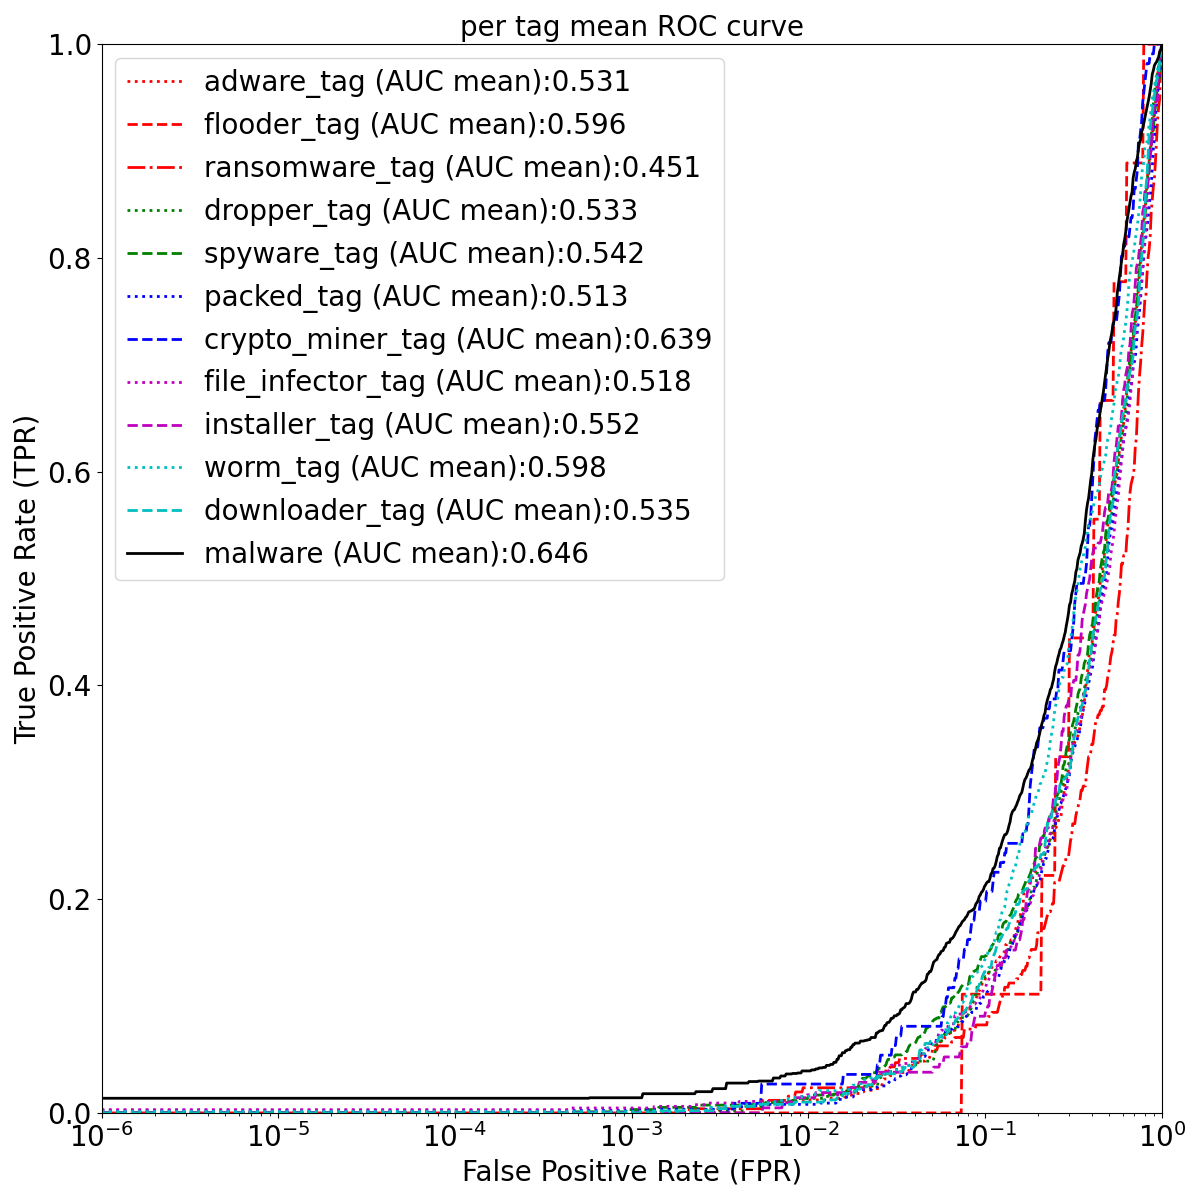
\includegraphics[width=0.7\textwidth]{./results/all_mean_roc_aloha.png}
        \vspace*{-0.2cm}
        \caption[Tags prediction task ALOHA mean ROC curve]{Mean ROC curve and AUC statistics of \textBF{ALOHA} model for the tags/labels. The line represents the \textit{mean} TPR at a given FPR. Statistics were computed over \textBF{3} training runs, each with random parameter initialization.}
        \label{fig:allMeanRocAloha}
    \end{figure}
}

\newcommand{\allMeanRocJointEmbedding}{
    \begin{figure}[H]
        \vspace*{-0.5cm}
        \centering
        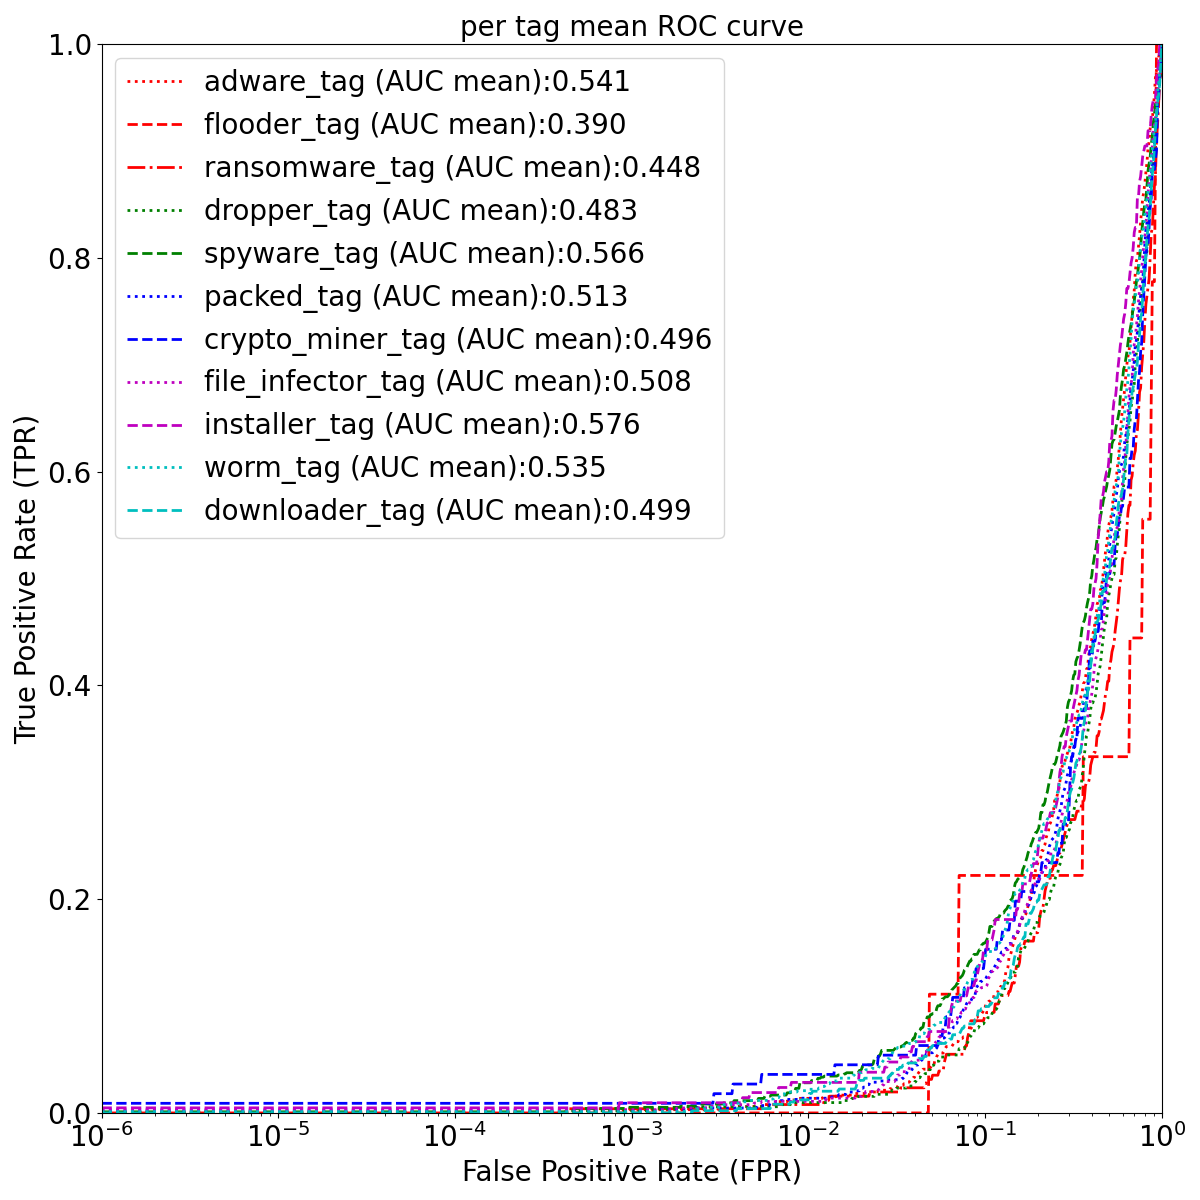
\includegraphics[width=0.7\textwidth]{./results/all_mean_roc_jointEmbedding.png}
        \vspace*{-0.2cm}
        \caption[Tags prediction task Joint Embedding mean ROC curve]{Mean ROC curve and AUC statistics of \textBF{Joint Embedding} model for all tags/labels. The line represents the \textit{mean} TPR at a given FPR. Statistics were computed over \textBF{3} training runs, each with random parameter initialization.}
        \label{fig:allMeanRocJointEmbedding}
    \end{figure}
}

\newcommand{\allMeanRocProposedModel}{
    \begin{figure}[H]
        \vspace*{-0.5cm}
        \centering
        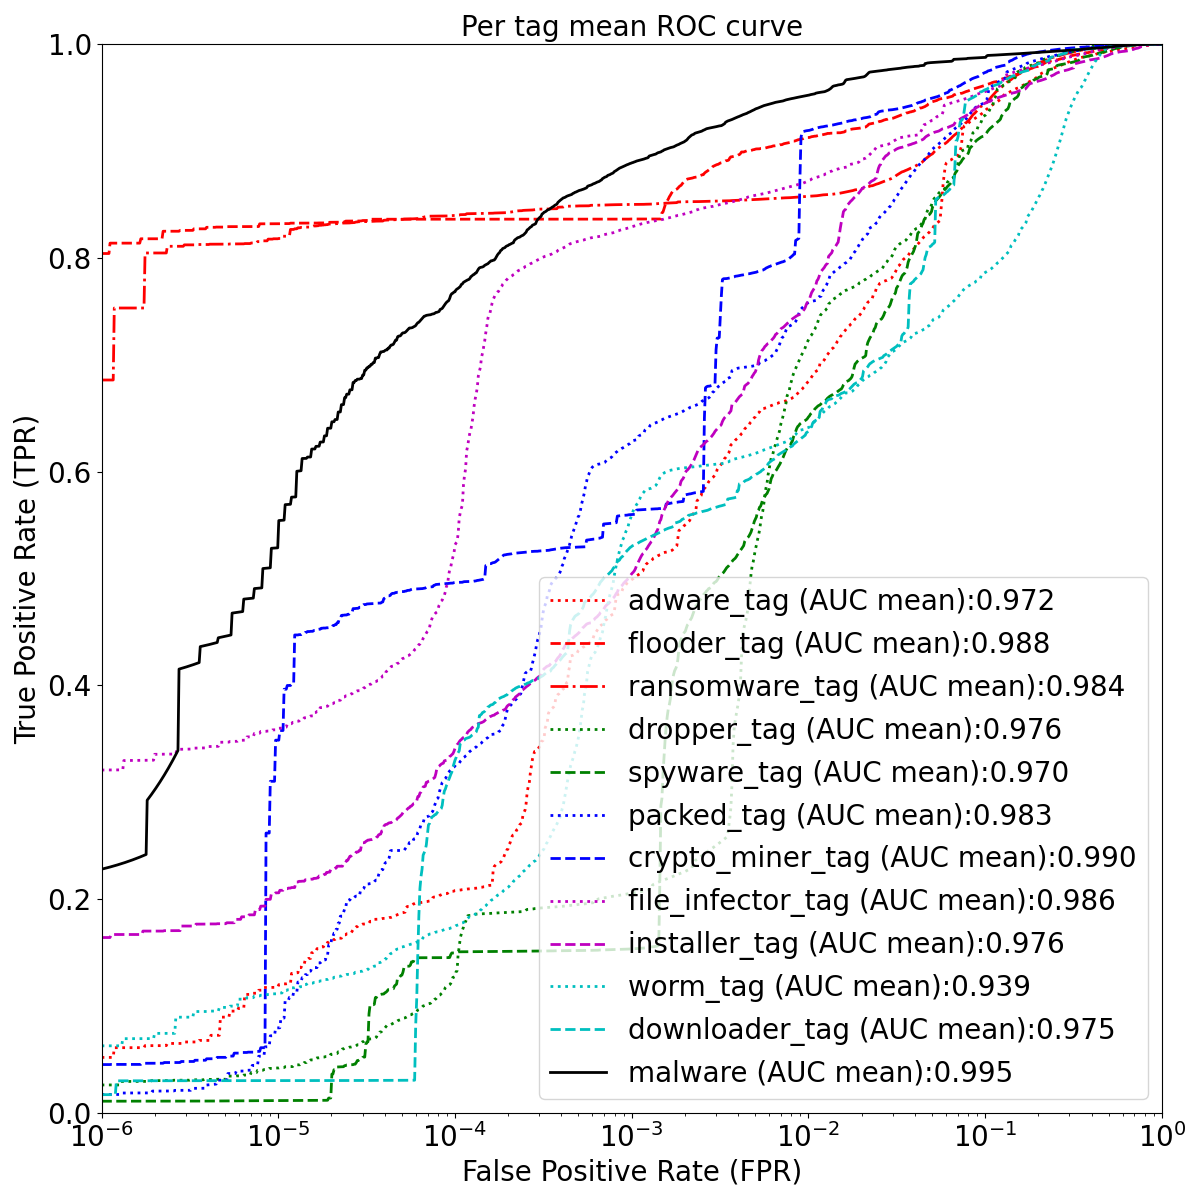
\includegraphics[width=0.7\textwidth]{./results/all_mean_roc_proposedModel.png}
        \vspace*{-0.2cm}
        \caption[Tags prediction task Proposed Model mean ROC curve]{Mean ROC curve and AUC statistics of \textBF{Proposed Model} for the tags/labels. The line represents the \textit{mean} TPR at a given FPR. Statistics were computed over \textBF{3} training runs, each with random parameter initialization.}
        \label{fig:allMeanRocProposedModel}
    \end{figure}
}